\section{\textit{Decision Trees}}

\subsection{\textit{Decision Trees}}

\textit{Decision Trees} (ook wel beslissingsbomen) worden vaak gebruikt op kleine, gestructureerde datasets en een categorische inputdata. Het werkt als een boomstructuur, waarbij we vertrekken van de \textit{root node} en vervolgens elke interne knoop (\textit{decision node}) een beslissing vertegenwoordigt op basis van een kenmerk, elke tak de uitkomst van een beslissing weergeeft, en elke bladknoop (\textit{leaf}) een eindklasse aangeeft.  Figuur \ref{fig:decision-tree} toont een voorbeeld van een beslissingsboom.

\begin{figure}[h]
	\centering
	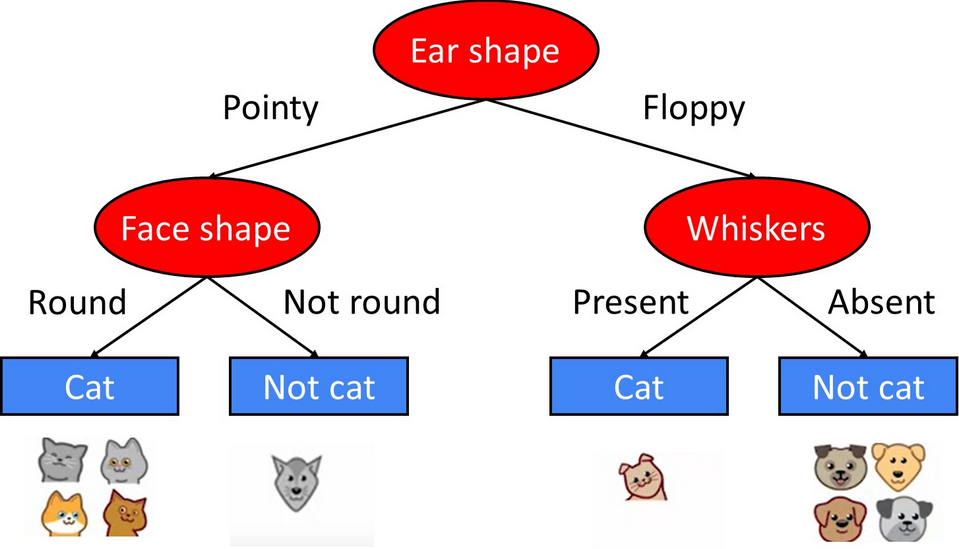
\includegraphics[width=0.5\textwidth]{images/29-decision-tree.png}
	\caption{Voorbeeld van een \textit{decision tree}}
	\label{fig:decision-tree}
\end{figure}
\noindent
We kunnen ons nu afvragen welke \textit{feature} we best gebruiken om een beslissing te maken. Dit zal de \textit{feature} zijn die de grootste zuiverheid (of kleinste onzuiverheid) oplevert. We zijn dus op zoek naar de perfecte split. Wanneer we dit toepassen op het voorbeeld van Figuur \ref{fig:decision-tree}, zien we dat bijvoorbeeld de gezichtsvorm zo een perfecte split oplevert aangezien alle dieren met een rond gezicht katten zijn en er geen enkele kat met een niet-rond gezicht is. \\
\newline
We kunnen ons ook de vraag stellen wanneer we stoppen met splitten. Hier zijn er een aantal mogelijkheden. We kunnen stoppen wanneer een node 100$\%$ uit één klasse bestaat. Er kan ook een maximum diepte aangegeven worden waarop we stoppen met splitten. Een andere optie is het instellen van een drempelwaarde voor de verbetering in zuiverheid of voor het aantal exemplaren per node om vervolgens te stoppen met splitten wanneer deze grens bereikt is.

\subsection{Entropie}

We kunnen entropie gebruiken om ze zuiverheid te meten. Stel dat $p_{0}$ onze fractie honden voorstelt en $p_{1}$ onze fractie katten. Het verband tussen beiden is dan:
\begin{equation}
	p_{0} = 1 - p_{1}
\end{equation}
\noindent
De entropie voor onze fractie katten kan als volgt berekend worden:
\begin{equation}
	H(p_{1}) = - p_{1} \log_{2} (p_{1}) - p_{0} \log_{2} (p_{0})
	= - p_{1} \log_{2} (p_{1}) - ( 1 - p_{1}) \log_{2} ( 1 - p_{1})
	\label{eq:entropy}
\end{equation}
\noindent
Figuur \ref{fig:entropy} toont het verloop van deze functie. We zien direct dat wanneer we een volledige verzameling honden of katten zouden hebben, onze entropie gelijk aan 0 zal zijn en dat wanneer onze split of 50$\%$ staat, onze entropie een maximale waarde van 1 zal bereiken.

\begin{figure}[h]
	\centering
	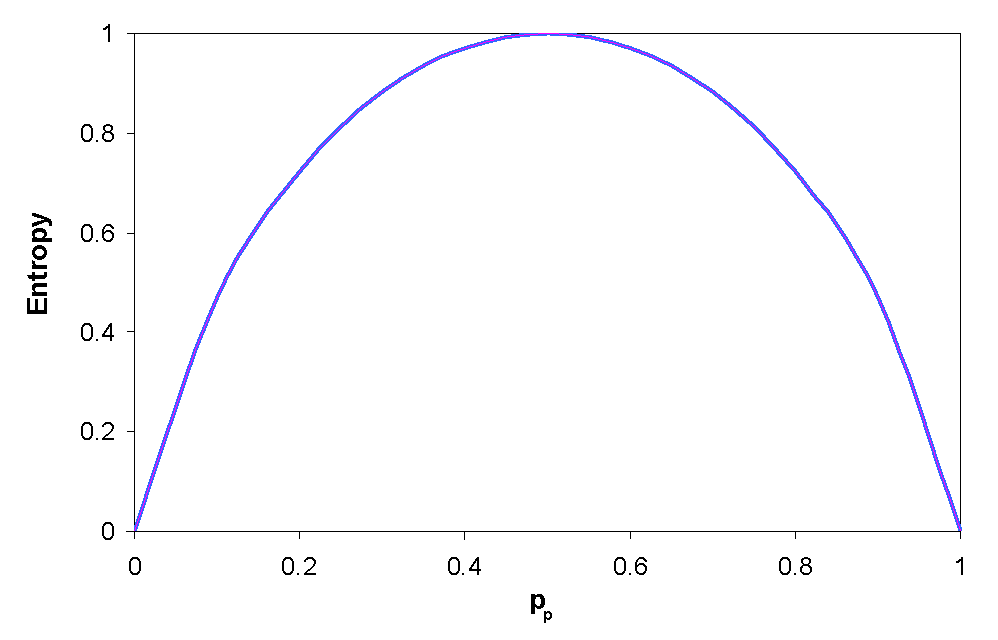
\includegraphics[width=0.5\textwidth]{images/30-entropy.png}
	\caption{Entropie}
	\label{fig:entropy}
\end{figure}

\paragraph{Entropie in Python}

We kunnen de entropie als volgt berekenen in Python:

\begin{lstlisting}
	def compute_entropy(y):
	    """
	    Computes the entropy for
	    Args:
	        y (ndarray): Numpy array indicating whether each example at a node is edible (`1`) or poisonous (`0`)
	    Returns:
	        entropy (float): Entropy at that node
	    """
	    entropy = 0.
	
	    if len(y) != 0:
	        p1 = len(y[y == 1]) / len(y)
	        if p1 != 0 and p1 != 1:
	            entropy = - p1 * numpy.log2(p1) - (1-p1) * numpy.log2(1-p1)
	        else:
	            entropy = 0
	
	    return entropy
\end{lstlisting}
\newpage
\subsection{\textit{Information gain}}

We kunnen nu op zoek gaan naar een manier om te kijken welke split de beste is. Dit zullen we doen met de \textit{information gain}. Stel dat we een split hebben zoals op Figuur \ref{fig:decision-tree-split}. Aan de linkerkant hebben we een zuiverheid van 0,8 en aan de rechterkant één van 0,2. We kunnen met behulp van formule \ref{eq:entropy} de entropie berekenen. Omwille van de symmetrie van Figuur \ref{fig:entropy} zal deze gelijk zijn voor beide fracties. Vervolgens kunnen we het gewogen gemiddelde van de entropie (ook wel gewogen \textit{entropy impurity}) berekenen. Dit doen we als volgt:

\begin{equation}
	w^{left} H(p_{1}^{left}) + w^{right} H(p_{1}^{right})
\end{equation}
\noindent
Voor de waarden uit ons voorbeeld, zal dit het volgende resultaat opleveren:
\begin{equation}
	\frac{5}{10} H(0,8) + \frac{5}{10} H(0,2) = \frac{5}{10} \cdot 0,72+ \frac{5}{10} \cdot 0,72 = 0,72
\end{equation}
\noindent
Deze waarden willen we zo laag mogelijk hebben en zullen we vervolgens gebruiken om de \textit{information gain} te berekenen. Dit doen we als volgt:
\begin{equation}
	IG = H(p_{1}^{root}) - (w^{left} H(p_{1}^{left}) + w^{right} H(p_{1}^{right}))
\end{equation}
\noindent
In ons voorbeeld hebben we aan onze \textit{root} evenveel katten als honden, wat betekent dat $p_{1}$ gelijk is aan 0,5 en de bijhorende entropie H(0,5) dus gelijk is aan 1. We krijgen dus de volgende \textit{information gain}:
\begin{equation}
	IG = H(0,5) - 0,72 = 1 - 0,72 = 0,28
\end{equation}
\noindent
Deze \textit{information gain} trachten we zo hoog mogelijk te krijgen. We kunnen dit deze berekening dus uitvoeren voor een aantal verschillende splits en op basis daarvan de split met de hoogste \textit{information gain} kiezen. 

\begin{figure}[h]
	\centering
	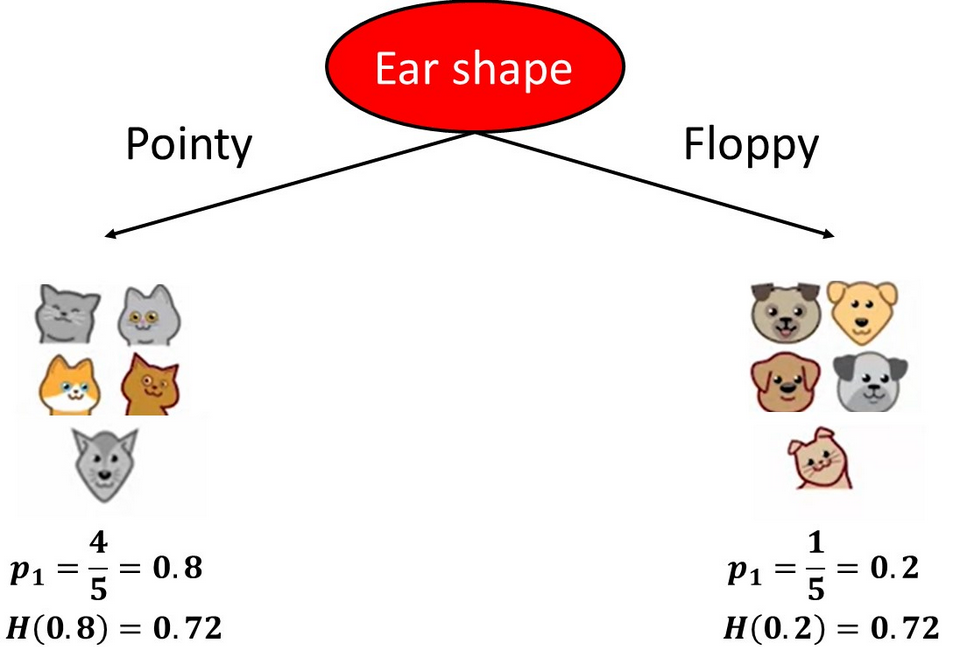
\includegraphics[width=0.75\textwidth]{images/31-decision-tree-split.png}
	\caption{Voorbeeld van een \textit{decision tree}}
	\label{fig:decision-tree-split}
\end{figure}
\newpage
\paragraph{\textit{Information gain} in Python}

We kunnen een split maken, de bijhorende \textit{information gain} berekenen en vervolgens de beste split selecteren. Dit kan met de volgende functies in Python:

\begin{lstlisting}
	def split_dataset(X, node_indices, feature):
	    """
	    Splits the data at the given node into left and right branches
	    Args:
	        X (ndarray):             Data matrix of shape(n_samples, n_features)
	        node_indices (list):     List containing the active indices. I.e, the samples being considered at this step.
	        feature (int):           Index of feature to split on
	    Returns:
	        left_indices (list):     Indices with feature value == 1
	        right_indices (list):    Indices with feature value == 0
	    """
	
	    left_indices = []
	    right_indices = []
	
	    for i in node_indices:
	        if (X[i][feature] :
	            left_indices.append(i) 
	        else: 
	            right_indices.append(i)
	
	    return left_indices, right_indices
\end{lstlisting}

\begin{lstlisting}
	def compute_information_gain(X, y, node_indices, feature):
	    """
	    Compute the information of splitting the node on a given feature
	    Args:
	        X (ndarray):            Data matrix of shape(n_samples, n_features)
	        y (array like):         list or ndarray with n_samples containing the target variable
	        node_indices (ndarray): List containing the active indices. I.e, the samples being considered in this step.
	    Returns:
	        cost (float):        Cost computed
	    """
	    # Split dataset
	    left_indices, right_indices = split_dataset(X, node_indices, feature)
	
	    # Some useful variables
	    X_node, y_node = X[node_indices], y[node_indices]
	    X_left, y_left = X[left_indices], y[left_indices]
	    X_right, y_right = X[right_indices], y[right_indices]
	
	    information_gain = 0
	
	    # Compute the entropy at the node
	    node_entropy = compute_entropy(y_node)
	    # Compute the entropy at the left branch
	    left_entropy = compute_entropy(y_left)
	    # Compute the entropy at the right branch
	    right_entropy = compute_entropy(y_right)
\end{lstlisting}

\begin{lstlisting}
	    # Compute the proportion of examples at the left branch
	    w_left = len(X_left) / len(X_node)
	
	    # Compute the proportion of examples at the right branch
	    w_right = len(X_right) / len(X_node)
	
	    # Compute weighted entropy from the split using w_left, w_right, left_entropy and right_entropy
	    weighted_entropy = w_left * left_entropy + w_right * right_entropy
	
	    # Compute the information gain as the entropy at the node minus the weighted entropy
	    information_gain = node_entropy - weighted_entropy
	
	    return information_gain
\end{lstlisting}

\begin{lstlisting}
	def get_best_split(X, y, node_indices):
	    """
	    Returns the optimal feature and threshold value to split the node data
	    Args:
	        X (ndarray):            Data matrix of shape(n_samples, n_features)
	        y (array like):         list or ndarray with n_samples containing the target variable
	        node_indices (ndarray): List containing the active indices. I.e, the samples being considered in this step.
	    Returns:
	        best_feature (int):     The index of the best feature to split
	    """
	    num_features = X.shape[1]
	
	    best_feature = -1
	    max_info_gain = 0
	
	    # Iterate through all features
	    for feature in range(num_features):
	        info_gain = compute_information_gain(X, y, node_indices, feature)
	
	        if info_gain > max_info_gain:  
	            max_info_gain = info_gain 
	            best_feature = feature
	
	    return best_feature
\end{lstlisting}
\noindent
Vervolgens kunnen we als volgt onze \textit{tree} recursief gaan opstellen, maar dit valt buiten de scope van dit vak:
\begin{lstlisting}
	tree = []
	
	def build_tree_recursive(X, y, node_indices, branch_name, max_depth, current_depth):
	    """
	    Build a tree using the recursive algorithm that split the dataset into 2 subgroups at each node.
	    This function just prints the tree.
	    """
\end{lstlisting}
\newpage
\begin{lstlisting}
	    """
	    Args:
	    X (ndarray):            Data matrix of shape(n_samples, n_features)
	    y (array like):         list or ndarray with n_samples containing the target variable
	    node_indices (ndarray): List containing the active indices. I.e, the samples being considered in this step.
	    branch_name (string):   Name of the branch. ['Root', 'Left', 'Right']
	    max_depth (int):        Max depth of the resulting tree.
	    current_depth (int):    Current depth. Parameter used during recursive call.
	    """
	
	    # Maximum depth reached - stop splitting
	    if current_depth == max_depth:
	        formatting = " "*current_depth + "-"*current_depth
	        print(formatting, "%s leaf node with indices" % branch_name, node_indices)
	        return
	
	    # Otherwise, get best split and split the data
	    # Get the best feature and threshold at this node
	    best_feature = get_best_split(X, y, node_indices)
	
	    formatting = "-"*current_depth
	    print("%s Depth %d, %s: Split on feature: %d" % (formatting, current_depth, branch_name, best_feature))
	
	    # Split the dataset at the best feature
	    left_indices, right_indices = split_dataset(X, node_indices, best_feature)
	    tree.append((left_indices, right_indices, best_feature))
	
	    # continue splitting the left and the right child. Increment current depth
	    build_tree_recursive(X, y, left_indices, "Left", max_depth, current_depth+1)
	    build_tree_recursive(X, y, right_indices, "Right", max_depth, current_depth+1)
\end{lstlisting}

\subsection{\textit{One-hot encoding}}

Het kan voorvallen dat we meer dan twee mogelijkheden hebben voor een bepaalde \textit{feature}. Om dit op te lossen, zullen we \textit{one-hot encoding} toepassen. Dit houdt in dat wanneer we een categorische \textit{feature} hebben die $k$ waarden kan hebben, we hier $k$ binaire \textit{features} van maken. Stel je voor dat onze \textit{ear shape} uit het voorbeeld niet alleen \textit{pointy} en \textit{floppy} kan zijn, maar ook \textit{oval}, dan zullen we deze \textit{feature} omvormen in 3 \textit{features} (\textit{pointy ears}, \textit{floppy ears} en \textit{oval ears}) die allemaal de waarde 0 of 1 zullen hebben. \\
\newline
We kunnen op dezelfde manier bijvoorbeeld de gezichtsvorm die rond of niet-rond is omvormen om hier een waarde 0 en 1 aan te koppelen.
\newpage
\subsection{\textit{Features} met een continue waarde}

Het kan ook voorvallen dat we in onze tabel een \textit{feature} hebben die een continue waarde heeft. Om deze in de \textit{decision tree} te betrekken, zullen we de data ordenen. Dit doen we door een drempelwaarde in te stellen en de split te maken op basis van of de waarde groter of kleiner is dan de gekozen drempel. Wanneer we $m$ datapunten hebben, kunnen we $m$ verschillende drempelwaarden kiezen en $m-1$ \textit{information gains} berekenen hiervoor.

\subsection{\textit{Regression Trees}}

We kunnen \textit{decision trees} ook gebruiken om een regressieprobleem op te lossen. We spreken dan van een \textit{regression tree}. Zo zouden we bijvoorbeeld ons algoritme kunnen gebruiken om het gewicht van onze kat te schatten. Dit doen we door onze nieuwe data toe te passen op de bestaande \textit{tree} en vervolgens het gemiddelde te nemen van de gewichten van de katten die in de \textit{leaf} zitten waarin we terechtkomen. Bij het opstellen van de \textit{regression tree} zullen we echter niet kijken naar de entropie, maar naar de variantie. De \textit{information gain} die we hier berekenen, is de reductie in variantie. Deze willen we opnieuw zo hoog mogelijk omdat we de variantie zo laag mogelijk willen. 

\subsection{\textit{Random Forest}-algoritme}

\textit{Decision trees} zijn hooggevoelig voor kleine veranderingen in de data. Hierdoor zijn ze niet robuust en gevoelig voor \textit{overfitting}. Om dit tegen te gaan, zullen we naar meerdere \textit{decision trees} tegelijkertijd kijken. Dit is het \textit{Random Forest}-algoritme. We kunnen nu kijken naar het label dat het meeste voorkomt voor ons datapunt. Dit principe noemen we \textit{majority voting}. We kunnen dit best een oneven aantal keer doen zodat we altijd een winnaar hebben. \\
\newline
Wanneer we onze \textit{decision trees} trainen, kunnen we gebruik maken van \textit{sampling with replacement}. Hierbij zullen we een aantal trainingsdata selecteren en deze vervolgens terug in onze dataset steken. Hierdoor worden onze verschillende modellen met verschillende training sets getraind en kan het voorvallen dat een trainingsdatapunt meerdere keren gebruikt wordt om een model te trainen. Dit zorgt voor een grotere diversiteit binnen ons model. We spreken ook van \textit{bagged decision trees}. \\
\newline
Het nadeel bij deze aanpak is dat wanneer $m$ groot is, we vaak wel alsnog dezelfde splits zullen krijgen bij de \textit{root node} en de eerste \textit{decision nodes}. Om dit tegen te gaan, kunnen we ook de beschikbare \textit{features} om een split te maken randomiseren, door telkens maar een aantal \textit{features} beschikbaar te maken en hier uit de kiezen. Een goede grote-orde voor het aantal \textit{features} in de deelverzameling is de wortel van het totaal aantal \textit{features}. Dit kan wel enkel als $n$ groot genoeg is.

\subsection{XGBoost}

XGBoost is een manier waarop we de foutief geclassificeerde datapunten meer kans geven om geselecteerd te worden in onze volgende training set. 
